\documentclass[letter, 9pt]{article}
\usepackage{fullpage}
\usepackage[margin=0.4in]{geometry}
\usepackage{graphicx}
\usepackage{caption}
\usepackage{subcaption}
\usepackage{amsmath}
\usepackage{listings}
\usepackage{float}
\usepackage{array,multirow}
\usepackage{tikz}
\usepackage{cancel}
\usepackage{listings}
\setcounter{MaxMatrixCols}{20}
\usetikzlibrary{arrows}
\pagenumbering{gobble}
\begin{document}
\noindent
\large \textbf{Rahul Ghosh} \hfill \textbf{Assignment\#3}\\
\normalsize Student ID: 5476965 \hfill CSci 5512\\

\section*{Question 1}
If we represent the Bayesian Network with matrices:
\begin{equation*}
    P(x_0) = 
    \begin{bmatrix}
        1/3\\
        1/3\\
        1/3
    \end{bmatrix}
    \quad
    P(x_{t+1}|x_t) = T =
    \begin{bmatrix}
        0.6 & 0.35 & 0.05 \\
        0.2 & 0.6 & 0.2 \\
        0 & 0.5 & 0.5
    \end{bmatrix}
    \quad
    P(e_t|x_t) = E_t =
    \begin{bmatrix}
        0 & 0 & 0 \\
        0 & 0.05 & 0 \\
        0 & 0 & 0.4
    \end{bmatrix}
    \quad
    P(\neg e_t|x_t) = E_t =
    \begin{bmatrix}
        1 & 0 & 0 \\
        0 & 0.95 & 0 \\
        0 & 0 & 0.6
    \end{bmatrix}
\end{equation*}
The filtering equation can be written with matrices as:
\begin{equation*}
    F_{t+1} = \alpha E_{t+1}T'F_t, \quad where\ F_0 = P(x_0)
\end{equation*}
\begin{itemize}
    \item[(1)] $P(x_1|e_1=``not flooded") = P(x_1| \neg e_1) = F_1 = \alpha E_1T'F_0 = 
    \begin{bmatrix}
        0.304472\\
        0.524263\\
        0.171265
    \end{bmatrix}$
    \item[(2)] $P(x_2|e_1=``not flooded", e_2=``not flooded") = P(x_2|\neg e_1, \neg e_2) = F_2 = \alpha E_2T'F_1 = 
    \begin{bmatrix}
        0.322213\\
        0.539477\\
        0.13831
    \end{bmatrix}$
    \item[(2)] $P(x_3|e_1=``not flooded", e_2=``not flooded", e_3=``flooded") = P(x_3| \neg e_1, \neg e_2, e_3) = F_1 = \alpha E_3T'F_2 = 
    \begin{bmatrix}
        0\\
        0.246533\\
        0.753467
    \end{bmatrix}$
\end{itemize}
The values are for low, med and high respectively. The code for filtering is as follows:
\begin{lstlisting}[language=Python]
    import numpy as np
    
    P_xt1_xt = np.reshape(np.array([[0.6, 0.35, 0.05], [0.2,0.6,0.2], [0,0.5,0.5]]),(3,3))
    P_et_xt = np.reshape(np.array([[0, 0, 0], [0, 0.05, 0], [0, 0, 0.4]]), (3, 3))
    P_notet_xt = np.reshape(np.array([[1, 0, 0], [0, 0.95, 0], [0, 0, 0.6]]), (3, 3))
    
    f = np.zeros((3,4))
    f[:,0] = np.array([1/3, 1/3, 1/3])
    
    val = np.reshape(np.matmul(np.matmul(P_notet_xt, np.transpose(P_xt1_xt)), f[:, 0]), (3))
    f[:,1] = val/np.sum(val)
    
    val = np.reshape(np.matmul(np.matmul(P_notet_xt, np.transpose(P_xt1_xt)), f[:,1]), (3))
    f[:,2] = val/np.sum(val)
    
    val = np.reshape(np.matmul(np.matmul(P_et_xt, np.transpose(P_xt1_xt)), f[:,2]), (3))
    f[:,3] = val/np.sum(val)
\end{lstlisting}

\newpage
\section*{Question 2} The filtering equation can be written with matrices as:
\begin{equation*}
    B_t = TE_{t+1}B_{t+1}, \quad where\ B_T = \begin{bmatrix}1\\1\\1\end{bmatrix}
\end{equation*}
Thus the smoothing equation is given as 
\begin{equation*}
    S_t = \alpha F_t B_t
\end{equation*}
\begin{itemize}
    \item[(1)] $P(x_1|e_1=``not flooded", e_2=``not flooded", e_3=``flooded") = P(x_1| \neg e_1, \neg e_2, e_3) = S_1 = \alpha F_1B_1 = 
    \begin{bmatrix}
        0.219015\\
        0.556865\\
        0.22412
    \end{bmatrix}$
    \item[(2)] $P(x_2|e_1=``not flooded", e_2=``not flooded", e_3=``flooded") = P(x_2| \neg e_1, \neg e_2, e_3) = S_2 = \alpha F_2B_2 = 
    \begin{bmatrix}
        0.117831\\
        0.578695\\
        0.303474
    \end{bmatrix}$
    \item[(2)] $P(x_3|e_1=``not flooded", e_2=``not flooded", e_3=``flooded") = P(x_3| \neg e_1, \neg e_2, e_3) = S_3 = \alpha F_3B_3 = 
    \begin{bmatrix}
        0\\
        0.246533\\
        0.753467
    \end{bmatrix}$
\end{itemize}
\begin{figure}[H]
    \minipage{0.33\textwidth}
        \centering
        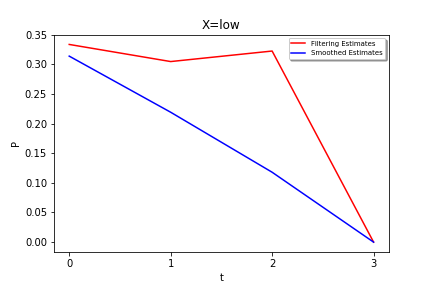
\includegraphics[width=\textwidth]{HW3/low.png}
    \endminipage\hfill
    \minipage{0.33\textwidth}
        \centering
        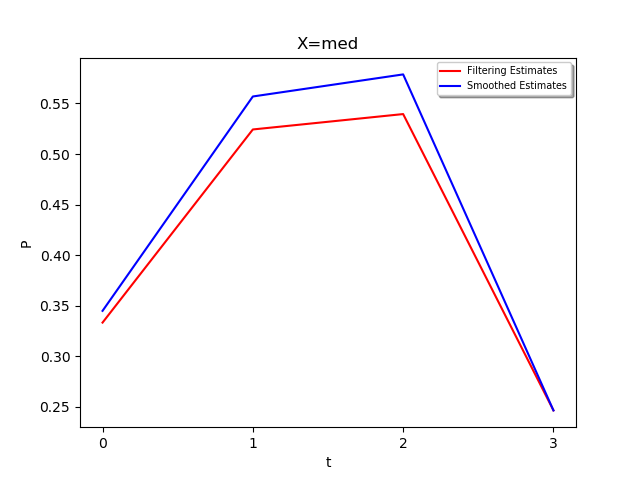
\includegraphics[width=\textwidth]{HW3/med.png}
    \endminipage\hfill
    \minipage{0.33\textwidth}
        \centering
        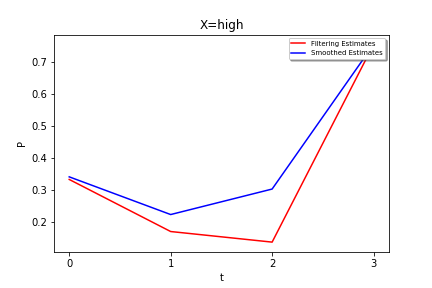
\includegraphics[width=\textwidth]{HW3/high.png}
    \endminipage\hfill
    \caption{Probability of filtered and smoothed estimates}
\end{figure}
The code for smoothing is as follows:
\begin{lstlisting}[language=Python]
    import numpy as np
    from numpy.linalg import inv

    P_xt1_xt = np.reshape(np.array([[0.6, 0.35, 0.05], [0.2, 0.6, 0.2], [0, 0.5, 0.5]]), (3, 3))
    P_et_xt = np.reshape(np.array([[0, 0, 0], [0, 0.05, 0], [0, 0, 0.4]]), (3, 3))
    P_notet_xt = np.reshape(np.array([[1, 0, 0], [0, 0.95, 0], [0, 0, 0.6]]), (3, 3))
    f = np.zeros((3,4))
    f[:,0] = np.array([1/3, 1/3, 1/3])
    h = np.zeros((3,4))
    h[:,-1] = np.array([1,1,1])
    S = np.zeros((3,4))
    val = np.reshape(np.matmul(np.matmul(P_notet_xt, np.transpose(P_xt1_xt)), f[:, 0]), (3))
    f[:,1] = val/np.sum(val)
    val = np.reshape(np.matmul(np.matmul(P_notet_xt, np.transpose(P_xt1_xt)), f[:,1]), (3))
    f[:,2] = val/np.sum(val)
    val = np.reshape(np.matmul(np.matmul(P_et_xt, np.transpose(P_xt1_xt)), f[:,2]), (3))
    f[:,3] = val/np.sum(val)
    val = np.reshape(np.matmul(np.matmul(P_xt1_xt, P_et_xt), h[:, 3]), (3))
    h[:,2] = val/np.sum(val)
    val = np.reshape(np.matmul(np.matmul(P_xt1_xt, P_notet_xt), h[:, 2]), (3))
    h[:,1] = val/np.sum(val)
    val = np.reshape(np.matmul(np.matmul(P_xt1_xt, P_notet_xt), h[:, 1]), (3))
    h[:,0] = val/np.sum(val)
    S = np.multiply(h, f)
    S = np.transpose(np.transpose(S))/np.transpose(sum(S))
\end{lstlisting}

\newpage
\section*{Question 3}
If we represent the Bayesian Network with matrices:
\begin{equation*}
    P(x_0) = 
    \begin{bmatrix}
        1/3\\
        1/3\\
        1/3
    \end{bmatrix}
    \quad
    P(x_{t+1}|x_t) = T =
    \begin{bmatrix}
        0.6 & 0.35 & 0.05 \\
        0.2 & 0.6 & 0.2 \\
        0 & 0.5 & 0.5
    \end{bmatrix}
    \quad
    P(e_t|x_t) = E_t =
    \begin{bmatrix}
        0 & 1\\
        0.05 & 0.95 \\
        0.4 & 0.6
    \end{bmatrix}
\end{equation*}
Using the matrices we create the MLE table using the following equation
\begin{equation*}
    MLE(t+1) = P(e_t|x_t)\max_{x_t} P(x_{t+1}|x_t) MLE(t)
\end{equation*}
For the given evidence: $e_1=“flooded”, e_2=“not flooded”, e_3=“not flooded”, e_4=“flooded”, e_5=“not flooded”$, we get the table as,
\begin{equation*}
    MLE = 
    \begin{bmatrix}
    0.333333333 & 0 & 0.002 & 0.00633333333 & 0 & 0.0001083\\
    0.333333333 & 0.01 & 0.0316666667 & 0.01805 & 0.0005415 & 0.0006859\\
    0.333333333 & 0.0666666667 & 0.02 & 0.006 & 0.001444 & 0.0004332
    \end{bmatrix}
\end{equation*}
Thus the sequence we get is $[x_0=low, x_1=high, x_2=med, x_3=med, x_4=high, x_5=med]$\\
For the given evidence: $e_1=“flooded”, e_2=“not flooded”, e_3=“not flooded”, e_4=“flooded”, e_5=“not flooded”, e_6="flooded"$, we get the table as,
\begin{equation*}
    MLE = 
    \begin{bmatrix}
    0.333333333 & 0 & 0.002 & 0.00633333333 & 0 & 0.0001083 & 0\\
    0.333333333 & 0.01 & 0.0316666667 & 0.01805 & 0.0005415 & 0.0006859 & 0.000020577\\
    0.333333333 & 0.0666666667 & 0.02 & 0.006 & 0.001444 & 0.0004332 & 0.00008664
    \end{bmatrix}
\end{equation*}
Thus the sequence we get is $[x_0=low, x_1=high, x_2=med, x_3=med, x_4=high, x_5=med, x_6=high]$\\
The code to find the Maximum Likelihood Estimate is as follows:
\begin{lstlisting}[language=Python]
    import numpy as np

    P_0 = np.array([1/3, 1/3, 1/3])
    P_xt1_xt = np.reshape(np.array([[0.6, 0.35, 0.05], [0.2, 0.6, 0.2], [0, 0.5, 0.5]]), (3, 3))
    P_et_xt = np.transpose(np.array([[0, 0.05, 0.4], [1, 0.95, 0.6]]))
    
    #Evidence till day 5
    T=5
    E = np.ones(T+1, dtype=int)
    E[[1,4]] = 0
    MLE = np.zeros((len(P_0), T+1), dtype=float)
    MLE[:,0] = P_0
    
    for t in range(1, T+1):
        MLE[:,t] = P_et_xt[:,E[t]] * np.amax((P_xt1_xt.T*MLE[:,t-1]).T, axis=0)
    val = np.argmax(MLE, axis=0)
    print(val)

    #Evidence till day 6
    T=6
    E = np.ones(T+1, dtype=int)
    E[[1,4,6]] = 0
    MLE = np.zeros((len(P_0), T+1), dtype=float)
    MLE[:,0] = P_0
    
    for t in range(1, T+1):
        MLE[:,t] = P_et_xt[:,E[t]] * np.amax((P_xt1_xt.T*MLE[:,t-1]).T, axis=0)
    val = np.argmax(MLE, axis=0)
    print(val)
\end{lstlisting}



\newpage
\section*{Question 4}Using N=100 particles and the particle filtering algorithm, we get the following distribution of particles,
\begin{equation*}
    \begin{bmatrix}
    38 & 19 & 24 & 0 & 0 & 1 & 19 & 31 & 21 & 0 & 4\\
    29 & 55 & 56 & 28 & 19 & 68 & 54 & 49 & 57 & 14 & 51\\
    33 & 26 & 20 & 72 & 81 & 31 & 27 & 20 & 22 & 86 & 45
    \end{bmatrix}
\end{equation*}
Therefore, $P(x_{10}|\neg e_1, \neg e_2, e_3, e_4, \neg e_5, \neg e_6, \neg e_7, \neg e_8, e_9) = \begin{bmatrix}0.4\\0.51\\0.45\end{bmatrix}$
The code for particle filtering is as follows:
\begin{lstlisting}[language=Python]
    import numpy as np
    import random
    
    def sample(N, prob):
        x = np.zeros(3)
        for i in range(N):
            rand_num = random.uniform(0, 1)
            if rand_num<=prob[0]:
                x[0] += 1
            elif rand_num <= prob[1]+prob[0]:
                x[1] += 1
            else:
                x[2] += 1
        return x
    
    P_0 = np.array([1/3, 1/3, 1/3])
    P_xt1_xt = np.reshape(np.array([[0.6, 0.35, 0.05], [0.2, 0.6, 0.2], [0, 0.5, 0.5]]), (3, 3))
    P_et_xt = np.array([[0, 0.05, 0.4], [1, 0.95, 0.6]])

    N = 100
    E = np.ones(11, dtype=int)
    E[[3,4,9]] = 0
    X = np.zeros((3,len(E)))
    
    X[:,0] = sample(N, P_0)
    for i in range(1, len(E)):
        X[:, i] = np.add(X[:, i], sample(int(X[0, i-1]), P_xt1_xt[0, :]))
        X[:, i] = np.add(X[:, i], sample(int(X[1, i-1]), P_xt1_xt[1, :]))
        X[:, i] = np.add(X[:, i], sample(int(X[2, i-1]), P_xt1_xt[2, :]))
        prob = np.multiply(X[:,i], P_et_xt[E[i],:])/np.sum(np.multiply(X[:,i], P_et_xt[E[i],:]))
        X[:,i] = sample(N,prob)
\end{lstlisting}

\newpage
\section*{Question 5}
$P(x_0) = \mathcal{N}(0,1) \implies \sigma_0^2=1$\\
$P(e_t|x_t) = \mathcal{N}(x_t,0.75) \implies \sigma_z^2=0.75$\\
The accuracy of our throw is $\sigma_x^2$\\
The variance at time t+1 is given by $\sigma_{t+1}^2 = \frac{(\sigma_t^2 + \sigma_x^2)\sigma_z^2}{\sigma_t^2 + \sigma_x^2 + \sigma_z^2}$\\
For the value of accuracy in the range [0, 100], the variance after 10 throws is plotted. We can see the variance after 10 throws is asymptotic at the value 0.744. Thus whatever be the value of accuracy, the variance after 10 throws will always be less than 10.

\begin{figure}[H]
    \centering
        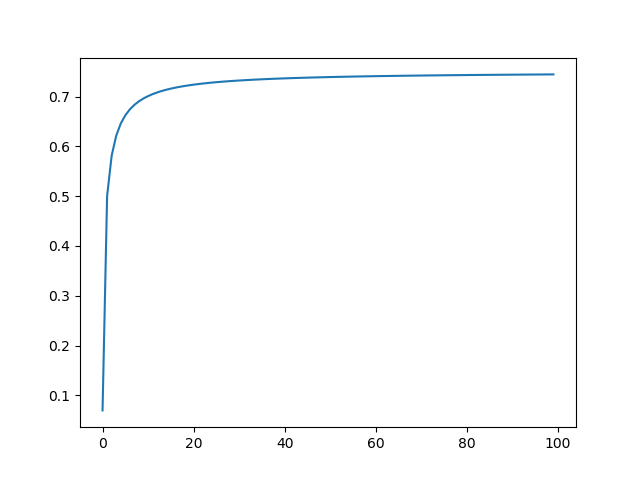
\includegraphics[width=\textwidth, height=0.3\textwidth]{HW3/variance.png}
\end{figure}

The code for computing the variance after 10 throws for a given accuracy is as follows:
\begin{lstlisting}[language=Python]
    import matplotlib.pyplot as plt
    import numpy as np
    
    sigma_osq = 1
    list_sigma_xsq = list(range(0,100))
    sigma_zsq = 0.75
    list_sigma_tsq = []
    
    for sigma_xsq in list_sigma_xsq:
        sigma_tsq = 1
        for i in range(1,11):
            sigma_t1sq = ((sigma_tsq + sigma_xsq)/(sigma_tsq + sigma_xsq + sigma_zsq))*sigma_zsq
            sigma_tsq = sigma_t1sq
        list_sigma_tsq.append(sigma_tsq)
\end{lstlisting}

\newpage
\section*{Question 6}
$P(X_0)=Uniform(-1,1) \qquad P(X_{t+1}|X_{t})=\mathcal{N}(x_t,\,1) \qquad P(e_t|x_t)=\mathcal{N}(x_t,\,0.5)$\\
i.e. $\sigma_x^2=1,\quad \sigma_z^2=\frac{1}{2}$\\
\begin{align*}
    P(x_1|z_1=0) & =\alpha P(z_1|x_1)\int_{-\infty}^{\infty}P(x_0)P(x_1|x_0) dx_0\\
    & = \alpha \frac{1}{\sqrt{2\pi\frac{1}{2}}}e^{-\frac{x_1^2}{2\times\frac{1}{2}}}\int_{-1}^{1}\frac{1}{\sqrt{2\pi}}e^{-\frac{(x_1-x_0)^2}{2}} dx_0
\end{align*}
Now the integeration is always less than 1. Therefore
\begin{align*}
P(x_1|z_1=0) & = \alpha \frac{1}{\sqrt{2\pi\frac{1}{2}}}e^{-\frac{x_1^2}{2\times\frac{1}{2}}}\cancelto{1}{\int_{-1}^{1}\frac{1}{\sqrt{2\pi}}e^{-\frac{(x_1-x_0)^2}{2}} dx_0}\\
P(x_1|z_1=0) & = \frac{1}{\sqrt{2\pi\frac{1}{2}}}e^{-\frac{x_1^2}{2\times\frac{1}{2}}}\\
P(x_1|z_1=0) & = \mathcal{N}(0,\frac{1}{2})(x_1)
\end{align*}
Therefore, $\mu_1=0\ and\ \sigma_1^2 = \frac{1}{2}$. The plot of $P(x_1|z_1=0)$ is shown in Figure 2.
\begin{align*}
    P(x_2|z_1=0, z_2=0) & =\alpha P(z_2|x_2)\int_{-\infty}^{\infty}P(x_1|x_0)P(x_1|z_1=0)dx_1\\
    & = \alpha \mathcal{N}(0,\frac{1}{2})\int_{-\infty}^{\infty}\mathcal{N}(0,1)\mathcal{N}(0,\frac{1}{2})dx_1
\end{align*}
All are gaussian distribution. Therefore now we can use the result derived in class, i.e.
\begin{equation*}
    \mu_{t+1} = \frac{(\sigma_t^2+\sigma_x^2)z_{t+1}+\sigma_x^2\mu_t}{\sigma_t^2+\sigma_x^2+\sigma_z^2} \quad \sigma_{t+1}^2=\frac{(\sigma_t^2+\sigma_x^2)\sigma_z^2}{\sigma_t^2+\sigma_x^2+\sigma_z^2}
\end{equation*}
where, $\sigma_t^2=\frac{1}{2},\ \sigma_z^2=\frac{1}{2},\ \sigma_x^2=1, z_2=0\ and\ \mu_t=0$\\
By substituting the values we get, $\mu_2=0,\ \sigma_2^2 = \frac{(\frac{1}{2}+1)\frac{1}{2}}{\frac{1}{2}+1+\frac{1}{2}} = \frac{3}{8}$
Therefore, $\mu_2=0\ and\ \sigma_2^2 = \frac{3}{8}$. The plot of $P(x_2|z_1=0, z_2=0)$ is shown in Figure 3.

As $t\rightarrow\infty$, the variance tends towards 0.36 as can be seen from the graph in figure 4.
\begin{figure}[H]
    \centering
        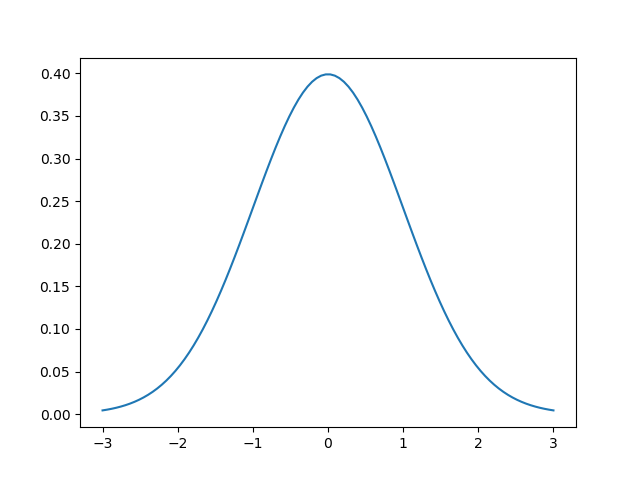
\includegraphics[width=\textwidth, height=0.4\textwidth]{HW3/t1.png}
    \caption{Distribution of $P(x_1|z_1=0)$}
\end{figure}

\begin{figure}[H]
    \centering
        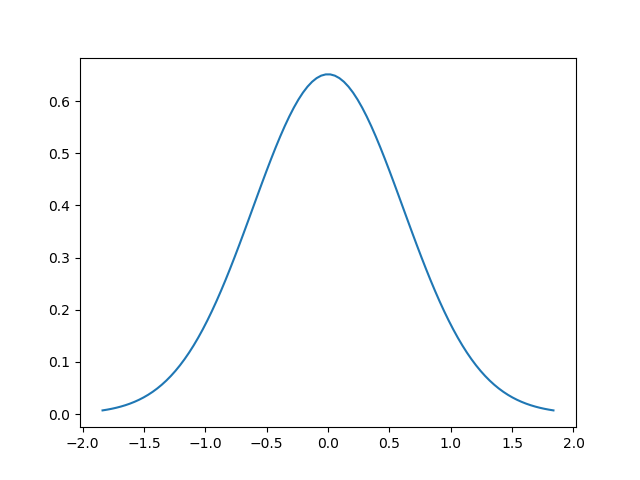
\includegraphics[width=\textwidth, height=0.4\textwidth]{HW3/t=2.png}
    \caption{Distribution of $P(x_2|z_1=0, z_2=0)$}
\end{figure}

\begin{figure}[H]
    \centering
        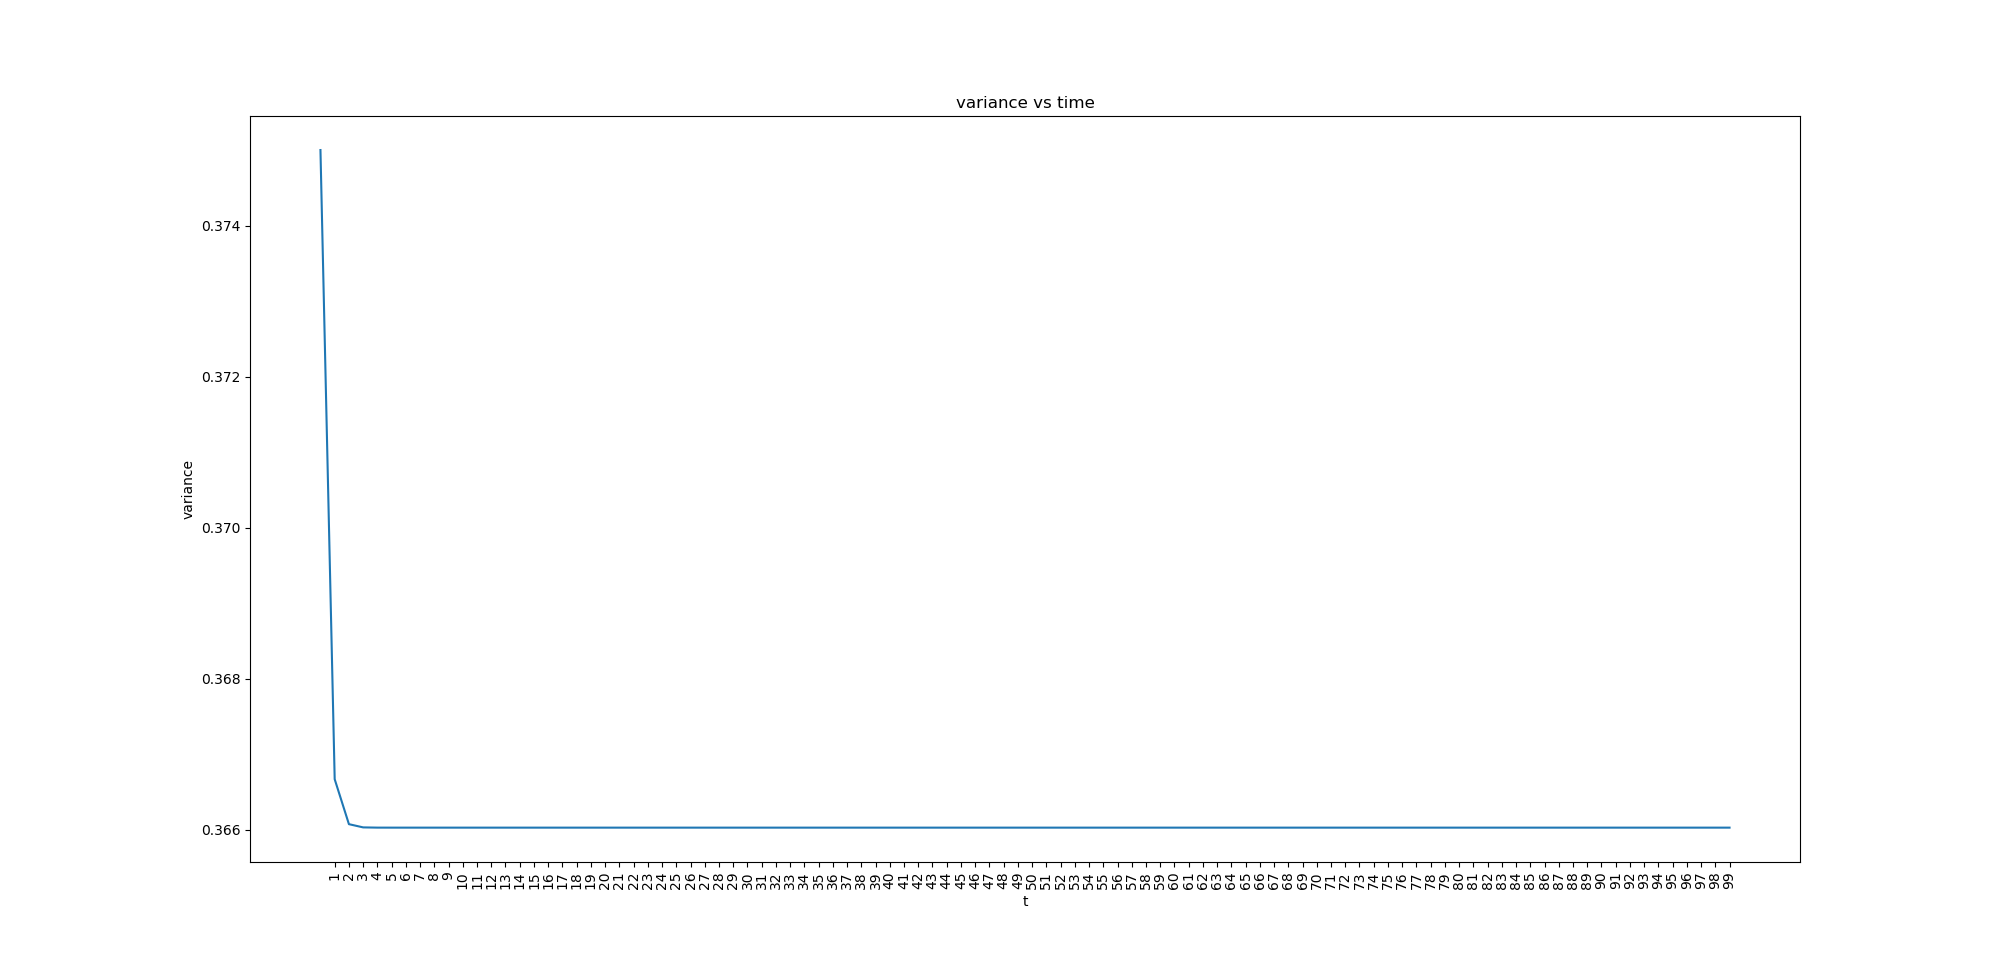
\includegraphics[width=\textwidth, height=0.4\textwidth]{HW3/variance_time.png}
    \caption{$\sigma_t^2\ vs\ time\ t$}
\end{figure}

\end{document}